\chapter{An Introduction to Teaching in Tanzania}
\section{A Good Teacher}
All of us have had teachers in the past that inspired us to learn.  Those teachers usually possess qualities such as kindness, a love for teaching, being lively and entertaining, motivation, having a passion and knowledge of subject, developing good rapport with the students, involving all students in teaching, correcting students without offending them, and knowing a student's weakness and strength.  These are qualities of a good teacher and ones we should strive for to make our lessons effective and inspirational.\\

A teacher has many roles in the classroom.  They are not just an instructor, but also as a manager, organizer, assessor, prompter, participant, tutor, facilitator, model, and observer.  A good teacher does not just lecture.  They manage students’ self learning, acting as a resource when necessary or participating alongside the student in learning.  Teachers are also role models for their students and can act as a counsellor if they observe something amiss in a student.\\

A teacher is a professional. Teaching is a noble profession.  Teachers develop the minds of future doctors, engineers, politicians, and parents.  Therefore, a teacher should always be a role model for their students. There are professional ethics to be followed by a teacher. Some practical points include:
\begin{itemize}
\item Being Punctual
\item Dressing Professionally
\item Preparing Lesson Plans
\item Respecting students 
\item Being a Leader
\item Being Honest
\end{itemize}

When we behave professionally and with the attitude of a teacher, our students and coworkers will respect us, regardless of age, gender, or nationality.  

\section{A Good Student}
Although it is unlikely that we will be blessed with all ``good'' students, we can encourage qualities of scholarship in our students.  A good learner is a student who is willing to listen and has a desire to experiment.  Good students are not afraid to ask questions and consider their own learning process.  By encouraging a desire to learn in our students, we can develop a more educated and thus more developed nation. \\

\begin{figure}[h!]
\centering
\setlength\fboxsep{0pt}
\setlength\fboxrule{2pt}
\fbox{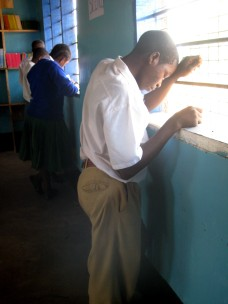
\includegraphics[scale=0.08]{./img/IMG_3697.JPG}} 
\end{figure}

When designing our lessons, we must consider our students' age, previous educational background, motivation, confidence, and language ability.  These may be different for each student.  As teachers we must be aware of these qualities and do our best to cater each lesson to the students’ abilities and needs.\\

Students learn in different ways.  Some learning types include: 
\begin{itemize}
\item verbal/linguistic
\item logical/mathematical
\item visual/spacial
\item musical/rhythmic
\item bodily/kinesthetic
\item interpersonal 
\item intrapersonal 
\end{itemize}



While teaching, we will face a variety of challenges that will prevent our students from learning.  Local culture or parents may not value education, discouraging children from studying or attending school.  Furthermore, students may may not relate education with work (or money), and therefore find it unimportant.  However, there are ways to motivate our students.  Such motivation for education could include future careers, study in other countries, improving the lives of themselves and their family, or bringing their country out of poverty.  

\section{Teaching in Tanzania}
Even for experienced teachers, teaching in Tanzania may prove to be a challenge.  The education system here is based on a British model that test students’ abilities with one final national examination.  Therefore, lessons tend to be focused on memorization rather than critical thinking.  \\

The Tanzanian education system is broken down into Primary, Secondary, and Tertiary education.  Primary education is compulsory, free, and begins around age 5 in Standard 1. In the mainland the medium of instruction is Kiswahili.  In Zanzibar, the students switch to English medium in Standard 5. Students will take a national exam in Standard 4 and again in Standard 7.  If they pass their Standard 7 exams (about 30 \% of students nationally), they will continue their education into Secondary School.  \\

Secondary education consists of Forms 1-6, with Forms 1-4 being Ordinary Level and Forms 5 and 6 being Advanced Level.  Students take a national exam (NECTA) in Form 2, but can continue their education whether they pass or fail.  Previously, students had to pass Form 2 exams to continue, but too many students were failing, so the government lifted this restriction.  In Form 4, students take another national exam.  If they pass in the top 3 Divisions, they may continue on to Advanced level.  If they get Division 4 or fail, they commonly find work as a primary school teacher, police officer, or attend vocational training schools.   Those who continue to Advanced Level will choose a three-course concentration for study.  In Form 6 they will take a final national exam on these three courses as well as General Studies.  If they do well, they will continue to University, if they do not, they usually become an Ordinary Level teacher or find private employment.\\

Tertiary Education is expanding rapidly in the country at the moment.  There are a wide variety of public and private universities, many of which offer Masters and even PhD programs.  Admittance into University is based solely on national examination scores and concentration in Advanced Level.  All applications are processed through an online application process.  University graduates may find work in the private sector, government or as instructors for Advanced Level.

\section{Common Challenges in a Tanzanian Classroom}
In any classroom a teacher will face common challenges like classroom management, diverse ability of students, and teaching with limited time and resources.  But Tanzanian education has its own unique challenges for teachers.  Because Tanzania was provided large amounts of foreign donor money to create schools, the education system grew explosively in the last 20 years.  Unfortunately, the Tanzanian government built secondary schools in each ward without securing resources or a teaching staff for those schools.  Thus, many schools volunteers teach at are under-resourced, both in materials and employees.  Because of limited staff, issues such as discipline, school management, and providing students with instruction for all subjects becomes a challenge.   Limited material resources affect both teaching aids in the classroom and retention of teachers.  Without electricity you cannot provide computer education or attract many new teachers.  However, there are ways to overcome these challenges which will be discussed further in Chapter 9 of this handbook.

\begin{center}
\setlength\fboxsep{0pt}
\setlength\fboxrule{2pt}
\fbox{
\includegraphics[scale=0.1]{./img/IMG_3643.JPG}}
\end{center}

\section{Benefits of Teaching in Tanzania	}
Just as there are unique challenges to this education system, there are also opportunities that are not present in other parts of the globe.  First and foremost, it is much easier to make a large impact here than in other parts of the world where teachers are abundant. Additionally, you may be the only native English speaker your students have ever known, thus, providing them with a unique experience to learn the language and pass their examinations.  Because the limited staff, most volunteers are also much more involved in the administration of the school, providing a unique opportunity to learn more about the education system and overcome some challenges the school may be facing.  Because of the culture and close community, teachers may also become very close with students and their families, developing life long friendships.  As with any situation, teaching in Tanzania has its ups and its downs.  We hope through your Peace Corps experience you will learn to make the most of the challenges and savour the successes.  

